\experiment{Singly Linked List Operations}{13/11/2023}

\section{Aim}
To implement a program for various operations on a singly linked list.

\section{Algorithm}
 {\fontfamily{lmtt}\selectfont

  \subsection{Structure Definition}
  Create a structure \texttt{Node} with the following attributes:
  \begin{enumerate}[label=\arabic*:,left=0pt]
    \item Integer \texttt{data} to store the data of the node.
    \item Pointer to \texttt{Node} \texttt{next} to store the address of the next node.
  \end{enumerate}

  \subsection{Function: \texttt{insertBegin}}
  Create a function \texttt{insertBegin(head, data)}:
  \begin{enumerate}[label=\arabic*:,left=0pt]
    \item \textbf{Start}
    \item Allocate memory for a new \texttt{Node} structure using \texttt{malloc}.
    \item Set \texttt{temp->next} to \texttt{head}.
    \item Set \texttt{temp->data} to \texttt{data}.
    \item Set \texttt{head} to \texttt{temp}.
    \item Return \texttt{head}.
    \item \textbf{Stop}
  \end{enumerate}

  \subsection{Function: \texttt{insertEnd}}
  Create a function \texttt{insertEnd(head, data)}:
  \begin{enumerate}[label=\arabic*:,left=0pt]
    \item \textbf{Start}
    \item Allocate memory for a new \texttt{Node} structure using \texttt{malloc}.
    \item Set \texttt{temp->data} to \texttt{data}.
    \item Set \texttt{temp->next} to \texttt{NULL}.
    \item If \texttt{head} is \texttt{NULL}, set \texttt{head} to \texttt{temp} and return \texttt{head}.
    \item Create a \texttt{Node} pointer \texttt{current} and set it to \texttt{head}.
    \item Loop while \texttt{current->next} is not \texttt{NULL}:
          \begin{enumerate}[label=2.\arabic*:, start=1]
            \item Set \texttt{current} to \texttt{current->next}.
          \end{enumerate}
    \item Set \texttt{current->next} to \texttt{temp}.
    \item Return \texttt{head}.
    \item \textbf{Stop}
  \end{enumerate}

  \subsection{Function: \texttt{display}}
  Create a function \texttt{display(head)}:
  \begin{enumerate}[label=\arabic*:,left=0pt]
    \item \textbf{Start}
    \item If \texttt{head} is \texttt{NULL}, print "The list is empty!!" and return.
    \item Print a newline.
    \item Create a \texttt{Node} pointer \texttt{current} and set it to \texttt{head}.
    \item Loop while \texttt{current} is not \texttt{NULL}:
          \begin{enumerate}[label=2.\arabic*:, start=1]
            \item Print \texttt{current->data} followed by a space.
            \item Set \texttt{current} to \texttt{current->next}.
          \end{enumerate}
    \item Print a newline.
    \item \textbf{Stop}
  \end{enumerate}

  \subsection{Function: \texttt{insertIndex}}
  Create a function \texttt{insertIndex(head, data, index)}:
  \begin{enumerate}[label=\arabic*:,left=0pt]
    \item \textbf{Start}
    \item Allocate memory for a new \texttt{Node} structure using \texttt{malloc}.
    \item Set \texttt{temp->data} to \texttt{data}.
    \item If \texttt{index == 1}, set \texttt{temp->next} to \texttt{head} and \texttt{head} to \texttt{temp}. Return \texttt{head}.
    \item Set integer \texttt{i} to 1.
    \item Set integer \texttt{done} to 0.
    \item Create a \texttt{Node} pointer \texttt{current} and a \texttt{Node} pointer \texttt{prev}.
    \item Loop while \texttt{current->next} is not \texttt{NULL}:
          \begin{enumerate}[label=2.\arabic*:, start=1]
            \item Set \texttt{prev} to \texttt{current}.
            \item Set \texttt{current} to \texttt{current->next}.
            \item If \texttt{i == index - 1}, set \texttt{prev->next} to \texttt{temp}, \texttt{temp->next} to \texttt{current}, and \texttt{done} to 1. Break the loop.
            \item Increment \texttt{i}.
          \end{enumerate}
    \item If \texttt{!done}, print "Index not valid!!".
    \item Return \texttt{head}.
    \item \textbf{Stop}
  \end{enumerate}

  \subsection{Function: \texttt{deleteBegin}}
  Create a function \texttt{deleteBegin(head)}:
  \begin{enumerate}[label=\arabic*:,left=0pt]
    \item \textbf{Start}
    \item If \texttt{head} is \texttt{NULL}, print "List is empty!!" and return \texttt{head}.
    \item Create a \texttt{Node} pointer \texttt{temp} and set it to \texttt{head}.
    \item Set \texttt{head} to \texttt{head->next}.
    \item Free \texttt{temp}.
    \item Return \texttt{head}.
    \item \textbf{Stop}
  \end{enumerate}

  \subsection{Function: \texttt{deleteEnd}}
  Create a function \texttt{deleteEnd(head)}:
  \begin{enumerate}[label=\arabic*:,left=0pt]
    \item \textbf{Start}
    \item If \texttt{head} is \texttt{NULL}, print "List is empty!!" and return \texttt{head}.
    \item If \texttt{head->next} is \texttt{NULL}, free \texttt{head}, set \texttt{head} to \texttt{NULL}, and return \texttt{head}.
    \item Create a \texttt{Node} pointer \texttt{current} and set it to \texttt{head}.
    \item Create a \texttt{Node} pointer \texttt{prev}.
    \item Loop while \texttt{current->next} is not \texttt{NULL}:
          \begin{enumerate}[label=2.\arabic*:, start=1]
            \item Set \texttt{prev} to \texttt{current}.
            \item Set \texttt{current} to \texttt{current->next}.
          \end{enumerate}
    \item Set \texttt{prev->next} to \texttt{NULL}.
    \item Free \texttt{current}.
    \item Return \texttt{head}.
    \item \textbf{Stop}
  \end{enumerate}

  \subsection{Function: \texttt{deleteIndex}}
  Create a function \texttt{deleteIndex(head, index)}:
  \begin{enumerate}[label=\arabic*:,left=0pt]
    \item \textbf{Start}
    \item If \texttt{head} is \texttt{NULL}, print "List is empty!!" and return \texttt{head}.
    \item If \texttt{index == 1}, create a \texttt{Node} pointer \texttt{temp} and set it to \texttt{head->next}. Free \texttt{head} and return \texttt{temp}.
    \item Set integer \texttt{i} to 1.
    \item Set integer \texttt{done} to 0.
    \item Create a \texttt{Node} pointer \texttt{current} and a \texttt{Node} pointer \texttt{prev}.
    \item Loop while \texttt{current->next} is not \texttt{NULL}:
          \begin{enumerate}[label=2.\arabic*:, start=1]
            \item Set \texttt{prev} to \texttt{current}.
            \item Set \texttt{current} to \texttt{current->next}.
            \item If \texttt{i == index - 1}, set \texttt{prev->next} to \texttt{current->next}, free \texttt{current}, and set \texttt{done} to 1. Break the loop.
            \item Increment \texttt{i}.
          \end{enumerate}
    \item If \texttt{!done}, print "Index not valid!!".
    \item Return \texttt{head}.
    \item \textbf{Stop}
  \end{enumerate}

  \subsection{Main Function}
  \begin{enumerate}[label=\arabic*:,left=0pt]
    \item \textbf{Start}
    \item Create a \texttt{Node} pointer \texttt{head} and set it to \texttt{NULL}.
    \item Set integer \texttt{ch}.
    \item Print menu options
    \item Loop while \texttt{ch != 8}:
          \begin{enumerate}[label=1.\arabic*:, start=1]
            \item Print "Choice: ".
            \item Take user input for \texttt{ch}.
            \item If \texttt{ch == 1}, call \texttt{display(head)}.
            \item If \texttt{ch == 2}:
                  \begin{enumerate}[label=3.\arabic*:, start=1]
                    \item Set integer \texttt{x}.
                    \item Print "Enter the data: ".
                    \item Take user input for \texttt{x}.
                    \item Call \texttt{insertBegin(head, x)} and assign the result to \texttt{head}.
                  \end{enumerate}
            \item If \texttt{ch == 3}:
                  \begin{enumerate}[label=4.\arabic*:, start=1]
                    \item Set integer \texttt{x}.
                    \item Print "Enter the data: ".
                    \item Take user input for \texttt{x}.
                    \item Call \texttt{insertEnd(head, x)} and assign the result to \texttt{head}.
                  \end{enumerate}
            \item If \texttt{ch == 4}:
                  \begin{enumerate}[label=5.\arabic*:, start=1]
                    \item Set integers \texttt{x} and \texttt{i}.
                    \item Print "Enter the data: ".
                    \item Take user input for \texttt{x}.
                    \item Print "Enter the index: ".
                    \item Take user input for \texttt{i}.
                    \item Call \texttt{insertIndex(head, x, i)} and assign the result to \texttt{head}.
                  \end{enumerate}
            \item If \texttt{ch == 5}, call \texttt{deleteBegin(head)} and assign the result to \texttt{head}.
            \item If \texttt{ch == 6}, call \texttt{deleteEnd(head)} and assign the result to \texttt{head}.
            \item If \texttt{ch == 7}:
                  \begin{enumerate}[label=8.\arabic*:, start=1]
                    \item Set integer \texttt{i}.
                    \item Print "Enter the index: ".
                    \item Take user input for \texttt{i}.
                    \item Call \texttt{deleteIndex(head, i)} and assign the result to \texttt{head}.
                  \end{enumerate}
            \item If \texttt{ch != 8} and \texttt{ch} is not one of the above options, print "Invalid option!".
          \end{enumerate}
    \item \textbf{Stop}
  \end{enumerate}
 }
\section{C Program}
\begin{lstlisting}[label={list:c_program:singly_linked_list}]
#include <stdlib.h>
#include <stdio.h>

typedef struct Node
{
  int data;
  struct Node *next;
} node;

node *insertBegin(node *head, int data);
node *insertEnd(node *head, int data);
node *insertIndex(node *head, int data, int index);
node *deleteBegin(node *head);
node *deleteEnd(node *head);
node *deleteIndex(node *head, int index);
void display(node *head);

int main()
{
  node *head = NULL;
  int ch;
  printf("1)Display\n2)InsertBegin\n3)InsertEnd\n4)InsertIndex\n5)deleteBegin\n6)deleteEnd\n7)deleteIndex\n8)Exit\n");
  do
  {
    printf("Choice: ");
    scanf("%d", &ch);
    if (ch == 1)
    {
      display(head);
    }
    else if (ch == 2)
    {
      int x;
      printf("\nEnter the data: ");
      scanf("%d", &x);
      printf("\n");
      head = insertBegin(head, x);
    }
    else if (ch == 3)
    {
      int x;
      printf("\nEnter the data: ");
      scanf("%d", &x);
      printf("\n");
      head = insertEnd(head, x);
    }
    else if (ch == 4)
    {
      int x, i;
      printf("\nEnter the data: ");
      scanf("%d", &x);
      printf("\nEnter the index: ");
      scanf("%d", &i);
      printf("\n");
      head = insertIndex(head, x, i);
    }
    else if (ch == 5)
    {
      head = deleteBegin(head);
    }
    else if (ch == 6)
    {
      head = deleteEnd(head);
    }
    else if (ch == 7)
    {
      int i;
      printf("\nEnter the index: ");
      scanf("%d", &i);
      printf("\n");
      head = deleteIndex(head, i);
    }
    else if (ch != 8)
    {
      printf("\nInvalid option!\n");
    }
  } while (ch != 8);
}

node *insertBegin(node *head, int data)
{
  /*printf("%d",data);*/
  node *temp;
  temp = (node *)malloc(sizeof(node));
  temp->next = head;
  temp->data = data;
  head = temp;
  return head;
}

node *insertEnd(node *head, int data)
{
  node *temp = (node *)malloc(sizeof(node));
  temp->data = data;
  temp->next = NULL;
  if (head == NULL)
  {
    head = temp;
    return head;
  }
  node *current = head;
  while (current->next != NULL)
  {
    current = current->next;
  }
  current->next = temp;
  return head;
}

void display(node *head)
{
  if (head == NULL)
  {
    printf("The list is empty!!\n");
    return;
  }
  printf("\n");
  node *current = head;
  while (current != NULL)
  {
    printf("%d ", current->data);
    current = current->next;
  }
  printf("\n");
}

node *insertIndex(node *head, int data, int index)
{
  node *temp = (node *)malloc(sizeof(node));
  temp->data = data;
  if (index == 1)
  {
    if (head != NULL)
      temp->next = head;
    head = temp;
    return head;
  }
  int i = 1;
  int done = 0;
  node *current = head;
  node *prev;
  while (current->next != NULL)
  {
    prev = current;
    current = current->next;
    if (i == index - 1)
    {
      prev->next = temp;
      temp->next = current;
      done = 1;
      break;
    }
    i++;
  }
  if (!done)
  {
    printf("Index not valid!!\n");
  }
  return head;
}

node *deleteBegin(node *head)
{
  if (head == NULL)
  {
    printf("List in empty!\n");
    return head;
  }
  node *temp = head;
  head = head->next;
  free(temp);
  return head;
}

node *deleteEnd(node *head)
{
  if (head == NULL)
  {
    printf("List in empty!\n");
    return head;
  }
  if (head->next == NULL)
  {
    free(head);
    head = NULL;
    return head;
  }
  node *current = head;
  node *prev;
  while (current->next != NULL)
  {
    prev = current;
    current = current->next;
  }
  prev->next = NULL;
  free(current);
  return head;
}

node *deleteIndex(node *head, int index)
{
  if (head == NULL)
  {
    printf("List is empty!!\n");
    return head;
  }
  if (index == 1)
  {
    node *temp = head->next;
    free(head);
    return temp;
  }
  int i = 1;
  int done = 0;
  node *current = head;
  node *prev;
  while (current->next != NULL)
  {
    prev = current;
    current = current->next;
    if (i == index - 1)
    {
      prev->next = current->next;
      free(current);
      done = 1;
      break;
    }
    i++;
  }
  if (!done)
  {
    printf("Index not valid!!\n");
  }
  return head;
}

\end{lstlisting}

\section{Output}
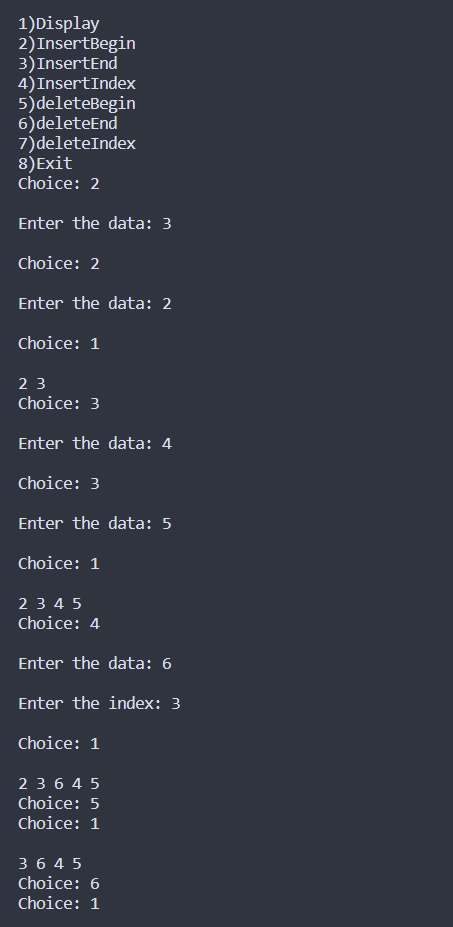
\includegraphics[]{Cycle_2/Outputs/LinkedList1.png}
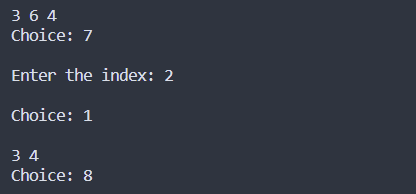
\includegraphics[]{Cycle_2/Outputs/LinkedList2.png}